\section{Feinentwurf}
\subsection{Vorüberlegungen}
Im Zuge der Erstellung des Feinentwurfs wird das Analysemodell des Grobentwurfs in fachlicher Hinsicher vervollständigt. Üblicherweise erfolgt dies durch Definition von Klassen, Attributen, Operationen und Assoziationen in einem Klassendiagramm. Das Self-Service-Terminal wird jedoch als Webapplikation in einem gesetzten Framework entwickelt und muss daher besonderen Anforderungen genügen.
Das Django Framework trennt Daten, Websitedesign und Logik voneinander, damit diese Elemente möglichst unabhängig von einander entwickelt werden können. Aufgrund dessen erscheint es sinnvoll den Feinentwurf nach der Struktur des Model-Template-View-Prinzips zu entwickeln. Struktur und Aufbau der MTV-Architektur sowie die Zusammenhänge der Elemente untereinander werden in \ref{fig:MVT_Erweitert} visualisiert.

\vspace{0,5cm}

\subsection{Model-Template-View-Prinzip}
Das Model-Template-View-Prinzip basiert auf einer möglichst losen Kopplung der Softwareelemente Model, Template und View. Die Aufgaben der entsprechenden Elemente unterscheiden sich dabei naturgemäß voneinander:\par 
\newpage 
\noindent \textbf{Models:} \par
\vspace{0,5cm}
\noindent Durch Models werden die Daten der Webapplikation gesteuert. Grundsätzlich gilt, dass jede Klasse der Modelle einer Relation in der zugrundeliegenden Datenbank entspricht. Die erstellten Klassen sind dabei Python Unterklassen der Klasse \textit{django.db.models.Model}. Aus den Modell Klassen können Objekte instanziiert werden. Die Attribute der generierten Klassen entsprechen dabei den Attributen der jeweiligen Relation. Zusammen ergeben sie also das Relationsschema. Anhand dieser Informationen steuert Django Anfragen an die Datenbank mithilfe einer \textit{database-access} API automatisch.\par
\vspace{1cm}
\noindent \textbf{Templates:}\par
\vspace{0,5cm}
\noindent Djangos Templates sind HTML-Dateien, welche durch Djangos eigene Templatesprache erweitert werden können. Sie enthalten damit Informationen über die Ausgabe statischer und dynamischer HTML Elemente. Die Struktur der Templates ist identisch zu gewöhnlichen HTML-Dateien. Die Django-Templatesprache erlaubt es aus einer Basis-HTML-Struktur zu vererben. Dadurch werden bestimmte Blöcke geändert. In for-Schleifen können HTML-Elemente wiederholt werden. Es ist außerdem möglich Variablen durch zustandsabhängige Werte zu ersetzen.

\newpage

\noindent \textbf{Views:}\par
\vspace{0,5cm}
\noindent Views sind Funktionen, welche eine http-Request übergeben bekommen und eine http-Response zurückgeben. Das View enthält dabei die dazu notwendige Logik um die Templates mit den vorgesehenen Daten zu rendern. Um die Projektstruktur möglichst einfach zu halten, legen wir auch andere anwendungsbezogene Logik in der view.py Datei ab. Nur Funktionen, die direkt mit den Model-Klassen interagieren werden in der model.py abgelegt.\par
\vspace{1cm}
\begin{figure}[htp]
    \centering
    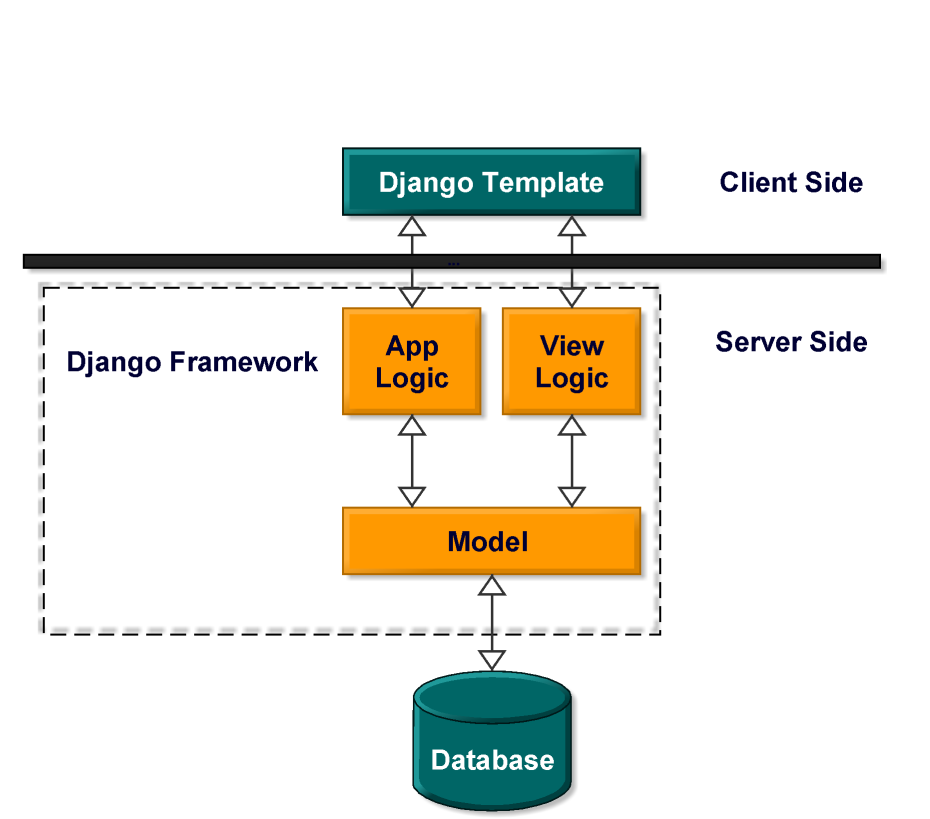
\includegraphics[width=12cm , height=11cm]{Kapitel/Bilder/MVT-Erweitert-Diesmalwirklich.PNG}
    \caption{Visualisierung des MVT-Prinzips im Django Framework}
    \label{fig:MVT_Erweitert}
\end{figure}
\newpage
\subsection{Architektur Entwurf}
Die Entwicklung des SST wird iterativ durchgeführt und orientiert sich an den zu erfüllenden Anforderungen. Die Architektur des Systems entwickelt sich daher im Geiste des gewählten agilen Vorgehensmodells Stück für Stück mit den implementierten Anforderungen. Das MTV-Prinzip gibt dabei die Struktur vor. 


